\part{Numerical Integrators}
\label{partNumericalMethods}

This analysis tool, which models alveolar geometry as a dodecahedron, requires numerical methods for the temporal integration of its constitutive equations (systems of first-order ODEs) and their governing equations of motion (systems of second-order ODEs), and for the spatial integrations of: length of line, area of surface, and volume of space that pertain to the various finite-element geometries required.  Results obtained at the Guass points need to be mapped out to their nodal locations, so extrapolation procedures that are consistent with the shape (interpolation) functions used are derived for the various elements and quadratures selected.

\section{ODE Solvers}

The constitutive equations used to describe our alveolar model present themselves as ordinary differential equations that need to be integrated, cf.\ \S\ref{secFE_CE}.  To this end, we employ the PECE (Predict, Evaluate, Correct, re-Evaluate) algorithms of Freed \cite{Freed17a} suitable for solving stiff systems of first- and second-order differential equations.  These methods are based upon Gear's well-known, second-order, backward, difference formula (BDF2) that appears in Eqns.~(\ref{1stOrderCorrector} \& \ref{velocityCorrector}) below.

Time $t$ is considered to be the independent variable, discretized over an interval in time $[t_0, t_N]$ for which $N$ solutions are to be extracted at nodes $n=1, 2, \ldots, N$ spaced at uniform intervals in time with a common step size of $\mathrm{d}t = (t_N - t_0)/N$ separating them, where time $t_0$ associates with the initial condition.

\subsection{PECE Solver for First-Order ODEs}
\label{sec:1stOrderPECE}

Let $\mathbf{x}(t)$ be a vector of independent control variables described in terms of time $t$, and let $\mathbf{y} (\mathbf{x})$ be a vector of dependent response variables obeying a differential equation of evolution $\dot{\mathbf{y}} = \mathbf{f} (\mathbf{x}, \mathbf{y}) \, \dot{\mathbf{x}}$, or equivalently $\mathrm{d} \mathbf{y} = \mathbf{f} (\mathbf{x}, \mathbf{y}) \, \dot{\mathbf{x}} \, \mathrm{d} t = \mathbf{f} (\mathbf{x}, \mathbf{y}) \, \mathrm{d}\mathbf{x}$, subject to an initial condition $\mathbf{y}_0 = \mathbf{y}(\mathbf{x}_0)$ where $\mathbf{x}_0 = \mathbf{x} (t_0)$ with matrix $\mathbf{f} (\mathbf{x}, \mathbf{y})$ establishing the constitutive response for the system.

The two-step method put forward here incrementally solves such an ODE, returning solutions associated with the next moment in time $t_{n+1}$, i.e., it acquires $\mathbf{y}_{n+1}$, given knowledge of the  previous $\mathbf{y}_{n-1}$ and current $\mathbf{y}_n$ solutions plus their rates $\dot{\mathbf{y}}_{n-1}$ and $\dot{\mathbf{y}}_n$, with the corrector also depending upon $\dot{\mathbf{y}}_{n+1}$; consequently, the corrector is an implicit method, which is the source of the method's stability properties.

\subsubsection{Start-Up Algorithm}

Multi-step methods are not self starting.  As such, Heun's method (a forward-Euler predictor with a trapezoidal corrector) is used to start this integrator; specifically,
\begin{subequations}
    \label{startUp1stOrderODEs}
    \begin{align}
    \mbox{} & \text{Predict} & 
    \mathbf{y}_1^p & = \mathbf{y}_0 + \dot{\mathbf{y}}_0 \, \mathrm{d}t + 
    \mathcal{O} \bigl( (\mathrm{d}t)^2 \bigr)
    \label{startUp1stOrderPredictor} \\
    \mbox{} & \text{Evaluate} & 
    \dot{\mathbf{y}}^p_1 & = \mathbf{f} (\mathbf{x}_1 , \mathbf{y}_1^p) \, 
    \dot{\mathbf{x}}_1
    \label{startUp1stEvaluate} \\
    \mbox{} & \text{Correct} &
    \mathbf{y}_1 & = \mathbf{y}_0 + \tfrac{1}{2} 
    \bigl( \dot{\mathbf{y}}_1^p + \dot{\mathbf{y}}_0 \bigr) \mathrm{d}t + 
    \mathcal{O} \bigl( (\mathrm{d}t)^3 \bigr)
    \label{startUp1stOrderCorrector} \\
    \mbox{} & \text{re-Evaluate} & 
    \dot{\mathbf{y}}_1 & = \mathbf{f} (\mathbf{x}_1 , \mathbf{y}_1) \,
    \dot{\mathbf{x}}_1 
    \label{startUp1stReEvaluate}
    \end{align}
\end{subequations}
wherein $\dot{\mathbf{y}}_0 = \mathbf{f}(\mathbf{x}_0, \mathbf{y}_0) \, \dot{\mathbf{x}}_0$.  The predictor is the forward Euler method, while the corrector is the trapezoidal rule.  The order of accuracy for a method (the exponent on $\mathrm{d}t$ in $\mathcal{O}$), as they appear in the above big $\mathcal{O}$ operators, pertains to a single step of integration.  The overall order of the method, when integrated over a sequence of steps, is one less than the exponent inside the $\mathcal{O}$ operator.  Therefore, Euler's method is first-order accurate, and Heun's method is second-order accurate.

\subsubsection{Two-Step ODE Solver}

The two-step method of Freed \cite{Freed17a} for solving first-order ODEs is
\begin{subequations}
    \label{1stOrderODEs}
    \begin{align}
    \mbox{} & \text{Predict} & 
    \mathbf{y}_{n+1}^p & = \tfrac{1}{3} 
    \bigl( 4 \mathbf{y}_n - \mathbf{y}_{n-1} \bigr) + 
    \tfrac{2}{3} \bigl( 2 \dot{\mathbf{y}}_n - \dot{\mathbf{y}}_{n-1} 
    \bigr) \mathrm{d}t + \mathcal{O} \bigl( (\mathrm{d}t)^3 \bigr)
    \label{1stOrderPredictor} \\
    \mbox{} & \text{Evaluate} & 
    \dot{\mathbf{y}}^p_{n+1} & = \mathbf{f} (\mathbf{x}_{n+1} , \mathbf{y}_{n+1}^p) \, \dot{\mathbf{x}}_{n+1}
    \label{1stOrderEvaluate} \\
    \mbox{} & \text{Correct} &
    \mathbf{y}_{n+1} & = \tfrac{1}{3} 
    \bigl( 4 \mathbf{y}_n - \mathbf{y}_{n-1} \bigr) + 
    \tfrac{2}{3} \dot{\mathbf{y}}^{p}_{n+1} \mathrm{d}t + 
    \mathcal{O} \bigl( (\mathrm{d}t)^3 \bigr)
    \label{1stOrderCorrector} \\
    \mbox{} & \text{re-Evaluate} & 
    \dot{\mathbf{y}}_{n+1} & = \mathbf{f} (\mathbf{x}_{n+1} , \mathbf{y}_{n+1}) \, 
    \dot{\mathbf{x}}_{n+1}
    \label{1stOrderReEvaluate}
    \end{align}
\end{subequations} 
whose corrector is the well-known BDF2 formula made popular by Gear, for which Freed has provided a predictor.  This method is second-order accurate in both its predictor and corrector.

Both the predictor and corrector of this PECE scheme have a solution $\mathbf{y}$ with a weight of 1, and a rate $\dot{\mathbf{y}}$ with a weight of $\tfrac{2}{3} \mathrm{d}t$; hence, this predictor\slash corrector pair is internally consistent, i.e., the predictor and corrector will produce the same result whenever they integrate over a constant $\dot{\mathbf{y}}$ field. 

The correct\slash re-evaluate (CE) steps of a PECE method are often iterated over until a convergence criterion is satisfied.  Such methods are typically denoted as $\text{PE}(\text{CE})^m$, where $m$ specifies the number of iterations imposed.


\subsection{A Relevant Example}

In our finite element implementation, a hypo-elastic material model \cite{Truesdell55} is introduced to describe the constitutive response of an alveolus whereby
\begin{displaymath}
    \dot{\boldsymbol{\sigma}} = \mathbf{M} ( \boldsymbol{\epsilon} , \boldsymbol{\sigma} ) \, \dot{\boldsymbol{\epsilon}} 
    \quad \text{or equivalently \cite{Noll55}} \quad
    \mathrm{d} \boldsymbol{\sigma} = \mathbf{M} ( \boldsymbol{\epsilon} , \boldsymbol{\sigma} ) \, \mathrm{d} \boldsymbol{\epsilon}
\end{displaymath} 
where $\boldsymbol{\epsilon}$ is a vector of thermo\-dynamic strains, $\boldsymbol{\sigma}$ is a vector of thermo\-dynamic stresses, and $\mathbf{M}$ is a square matrix comprised of their tangent moduli, which can depend upon both stress and strain in our application; specifically,
\begin{displaymath}
   \boldsymbol{\sigma}_{1D} = \{ \eta , s \}^{\mathsf{T}} , \quad
   \boldsymbol{\sigma}_{2D} = \{ \eta , s^{\pi} , s^{\sigma} , s^{\tau} \}^{\mathsf{T}} , \quad
   \boldsymbol{\sigma}_{3D} = \{ \eta , \Pi , \sigma_1 , \sigma_2 , \tau_1 , \tau_2 , \tau_3 \}^{\mathsf{T}}
\end{displaymath}
where $\eta$ is entropy and the rest of its constituents are stress attributes.  Their thermo\-dynamic conjugates are the control variables
\begin{displaymath}
\boldsymbol{\epsilon}_{1D} = \{ \theta , e \}^{\mathsf{T}} , \quad
\boldsymbol{\epsilon}_{2D} = \{ \theta , \xi , \varepsilon , \gamma \}^{\mathsf{T}} , \quad
\boldsymbol{\epsilon}_{3D} = \{ \theta , \Xi , \varepsilon_1 , \varepsilon_2 , \gamma_1 , \gamma_2 , \gamma_3 \}^{\mathsf{T}}
\end{displaymath}
where $\theta$ is temperature and the rest of its constituents are strain attributes.  In the 2- and 3-D cases, these stress\slash strain attributes arise from Gram-Schmidt decompositions of their respective deformation gradients (cf.\ Sections~\ref{secQR2D}, \ref{secConjugatePairs} and \ref{secFE_CE}).  Constructing tangent moduli $\mathbf{M} ( \boldsymbol{\epsilon} , \boldsymbol{\sigma} )$ is the topic of Part~\ref{partConstitutive}.  Both $\boldsymbol{\sigma}$ and $\mathrm{d} \boldsymbol{\sigma} = \mathbf{M} \, \mathrm{d} \boldsymbol{\epsilon}$ arise in the construction of our stiffness matrices, cf.\ \S\ref{secStiffnessMatrices}.

Equation (\ref{startUp1stOrderODEs}) is used to take the first step of integration; specifcally, 
\begin{subequations}
    \notag
    \begin{align}
    \mbox{} & \text{Predict} & 
    \boldsymbol{\sigma}_1^p & = \boldsymbol{\sigma}_0 + \dot{\boldsymbol{\sigma}}_0 \, \mathrm{d}t \\
    \mbox{} & \text{Evaluate} & 
    \dot{\boldsymbol{\sigma}}^p_1 & = \mathbf{M} ( \boldsymbol{\epsilon} , \boldsymbol{\sigma}_1^p ) \, \dot{\boldsymbol{\epsilon}}_1 \\
    \mbox{} & \text{Correct} &
    \boldsymbol{\sigma}_1 & = \boldsymbol{\sigma}_0 + \tfrac{1}{2} 
    \bigl( \dot{\boldsymbol{\sigma}}_1^p + 
    \dot{\boldsymbol{\sigma}}_0 \bigr) \mathrm{d} t \\
    \mbox{} & \text{re-Evaluate} & 
    \dot{\boldsymbol{\sigma}}_1 & = \mathbf{M} ( \boldsymbol{\epsilon}_1 , \boldsymbol{\sigma}_1 ) \, \dot{\boldsymbol{\epsilon}}_1
    \end{align}
\end{subequations}
where $\dot{\boldsymbol{\sigma}}_0 = \mathbf{M} ( \boldsymbol{\epsilon}_0 , \boldsymbol{\sigma}_0 ) \, \dot{\boldsymbol{\epsilon}}_0$.  The remaining steps of integration follow according to Eqn.~(\ref{1stOrderODEs}); specifically,
\begin{subequations}
    \notag
    \begin{align}
    \mbox{} & \text{Predict} & 
    \boldsymbol{\sigma}_{n+1}^p & = \tfrac{1}{3} 
    \bigl( 4 \boldsymbol{\sigma}_n - \boldsymbol{\sigma}_{n-1} \bigr) + 
    \tfrac{2}{3} \bigl( 2 \, \dot{\boldsymbol{\sigma}}_n - 
    \dot{\boldsymbol{\sigma}}_{n-1} \bigr) \mathrm{d} t \\
    \mbox{} & \text{Evaluate} & 
    \dot{\boldsymbol{\sigma}}^p_{n+1} & = \mathbf{M} ( \boldsymbol{\epsilon}_{n+1} , \boldsymbol{\sigma}_{n+1}^p ) \, \dot{\boldsymbol{\epsilon}}_{n+1} \\
    \mbox{} & \text{Correct} &
    \boldsymbol{\sigma}_{n+1} & = \tfrac{1}{3} 
    \bigl( 4 \boldsymbol{\sigma}_n - \boldsymbol{\sigma}_{n-1} \bigr) + 
    \tfrac{2}{3} \, \dot{\boldsymbol{\sigma}}^{p}_{n+1} \, \mathrm{d}t \\
    \mbox{} & \text{re-Evaluate} & 
    \dot{\boldsymbol{\sigma}}_{n+1} & = \mathbf{M} ( \boldsymbol{\epsilon}_{n+1} , 
    \boldsymbol{\sigma}_{n+1} ) \, \dot{\boldsymbol{\epsilon}}_{n+1}
    \end{align}
\end{subequations} 
whose strain rates $\dot{\boldsymbol{\epsilon}}$ are computed according to \S\ref{secFE_CE}.


\subsection{PECE Solver for Second-Order ODEs}
\label{sec:2ndOrderPECE}

Now let $\mathbf{u}$ denote a vector of dependent variables obeying a differential equation of evolution $\mathrm{d}^2 \mathbf{u}(t) / \mathrm{d} t^2 = \ddot{\mathbf{u}} = \mathbf{f} (t, \mathbf{u}, \dot{\mathbf{u}})$ subjected to the pair of initial conditions $\mathbf{u}_0 = \mathbf{u}(t_0)$ and $\dot{\mathbf{u}}_0 = \dot{\mathbf{u}}(t_0)$.  One may think of $\mathbf{u}$ as being displacements whose rates $\dot{\mathbf{u}}$ are velocities $\mathbf{v}$, with $\ddot{\mathbf{u}} = \dot{\mathbf{v}}$ representing their accelerations $\mathbf{a}$. 

The two-step method put forward here incrementally solves such an ODE, returning solutions associated with the next moment in time $t_{n+1}$ for both displacement $\mathbf{u}_{n+1}$ and velocity $\dot{\mathbf{u}}_{n+1}$.  To update the displacement to $\mathbf{u}_{n+1}$, the predictor requires knowledge of the previous fields $\mathbf{u}_{n-1}$, $\dot{\mathbf{u}}_{n-1}$ and $\ddot{\mathbf{u}}_{n-1}$ plus the current fields $\mathbf{u}_n$, $\dot{\mathbf{u}}_n$ and $\ddot{\mathbf{u}}_n$, with the corrector also requiring knowledge of $\dot{\mathbf{u}}_{n+1}$ and $\ddot{\mathbf{u}}_{n+1}$.  Likewise, to update the velocity to $\dot{\mathbf{u}}_{n+1}$, the predictor requires knowledge of the previous fields $\dot{\mathbf{u}}_{n-1}$ and $\ddot{\mathbf{u}}_{n-1}$ plus the current fields $\dot{\mathbf{u}}_n$ and $\ddot{\mathbf{u}}_n$, with the corrector also requiring knowledge of $\ddot{\mathbf{u}}_{n+1}$.  Both predictors are explicit, and both correctors are implicit.  It is this implicit quality that provides numeric stability for the integrator.

\subsubsection{Start-Up Algorithm}

Again, multi-step methods are not self starting, so a one-step method is needed to take the first step of integration; specifically, we employ
\begin{subequations}
    \label{pairedStartUp}
    \begin{align}
    \mbox{} & \text{Predict} & 
    \mathbf{u}_1^p & = \mathbf{u}_0 + \dot{\mathbf{u}}_0 \, \mathrm{d}t +
    \tfrac{1}{2} \ddot{\mathbf{u}}_0 (\mathrm{d}t)^2 + \mathcal{O} \bigl( ( \mathrm{d}t )^3 \bigr)
    \label{startupDisplacementPredictor} \\
    \mbox{} & &
    \dot{\mathbf{u}}^p_1 & = 
    \dot{\mathbf{u}}_0 + \ddot{\mathbf{u}}_0 \, \mathrm{d}t + 
    \mathcal{O} \bigl( ( \mathrm{d}t )^2 \bigr) 
    \label{startUpVelocityPredictor} \\
    \mbox{} & \text{Evaluate} &
    \ddot{\mathbf{u}}^p_1 & = \mathbf{f} (t_1, \mathbf{u}^p_1, \dot{\mathbf{u}}^p_1)
    \label{startUpEvaluate} \\
    \mbox{} & \text{Correct} &
    \mathbf{u}_1 & = \mathbf{u}_0 + \tfrac{1}{2} 
    ( \dot{\mathbf{u}}^p_1 + \dot{\mathbf{u}}_0 ) \mathrm{d}t -
    \tfrac{1}{12} ( \ddot{\mathbf{u}}^p_1 - 
    \ddot{\mathbf{u}}_0 ) (\mathrm{d}t)^2 + \mathcal{O} \bigl( (\mathrm{d}t)^4 \bigr) 
    \label{startupDisplacementCorrector} \\
    \mbox{} & &
    \dot{\mathbf{u}}_1 & = \dot{\mathbf{u}}_0 + \tfrac{1}{2} 
    ( \ddot{\mathbf{u}}_1^p + \ddot{\mathbf{u}}_0 ) \mathrm{d}t + 
    \mathcal{O} \bigl( (\mathrm{d}t)^3 \bigr)
    \label{startUpVelocityCorrector} \\
    \mbox{} & \text{re-Evaluate} &
    \ddot{\mathbf{u}}_1 & = \mathbf{f} (t_1, \mathbf{u}_1, \dot{\mathbf{u}}_1) 
    \label{startUpReEvaluate}
    \end{align}
\end{subequations}
wherein $\ddot{\mathbf{u}}_0 = \mathbf{f}(t_0, \mathbf{u}_0, \dot{\mathbf{u}}_0)$ and $t_1 = t_0 + \mathrm{d}t$. 


\subsubsection{Two-Step ODE Solver}

The two-step method of Freed \cite{Freed17a} for solving second-order ODEs is
\begin{subequations}
    \label{pairedMethods}
    \begin{align}
    \mbox{} & \text{Predict} &
    \mathbf{u}_{n+1}^p & = \tfrac{1}{3} (
    4 \mathbf{u}_n - \mathbf{u}_{n-1} ) + 
    \tfrac{1}{6} ( 3 \dot{\mathbf{u}}_n + 
    \dot{\mathbf{u}}_{n-1} ) \mathrm{d}t \notag \\ 
    \mbox{} & & & \qquad + 
    \tfrac{1}{36} ( 31 \ddot{\mathbf{u}}_n - 
    \ddot{\mathbf{u}}_{n-1} ) (\mathrm{d}t)^2 + 
    \mathcal{O} \bigl( (\mathrm{d}t)^4 \bigr) 
    \label{displacementPredictor} \\
    \mbox{} & &
    \dot{\mathbf{u}}_{n+1}^p & = \tfrac{1}{3} 
    ( 4 \dot{\mathbf{u}}_n - \dot{\mathbf{u}}_{n-1} ) + 
    \tfrac{2}{3} ( 2\ddot{\mathbf{u}}_n - \ddot{\mathbf{u}}_{n-1} )
    \mathrm{d}t + \mathcal{O} \bigl( (\mathrm{d}t)^3 \bigr)
    \label{velocityPredictor} \\
    \mbox{} & \text{Evaluate} &
    \ddot{\mathbf{u}}^p_{n+1} & = \mathbf{f} (t_{n+1}, \mathbf{u}^p_{n+1}, \dot{\mathbf{u}}^p_{n+1}) 
    \label{2ndEvaluate} \\
    \mbox{} & \text{Correct} & 
    \mathbf{u}_{n+1} & = \tfrac{1}{3} (
    4  \mathbf{u}_n - \mathbf{u}_{n-1} ) +
    \tfrac{1}{24} ( \dot{\mathbf{u}}^p_{n+1} +
    14 \dot{\mathbf{u}}_n + \dot{\mathbf{u}}_{n-1} ) \mathrm{d}t 
    \notag \\
    \mbox{} & & & \qquad +
    \tfrac{1}{72} ( 10 \ddot{\mathbf{u}}^p_{n+1} + 
    51 \ddot{\mathbf{u}}_n - \ddot{\mathbf{u}}_{n-1} ) (\mathrm{d}t)^2 + 
    \mathcal{O} \bigl( (\mathrm{d}t)^4 \bigr)
    \label{displacementCorrector} \\ 
    \mbox{} & &
    \dot{\mathbf{u}}_{n+1} & = \tfrac{1}{3} 
    ( 4 \dot{\mathbf{u}}_n - \dot{\mathbf{u}}_{n-1} ) + 
    \tfrac{2}{3} \ddot{\mathbf{u}}^p_{n+1} \, \mathrm{d}t + 
    \mathcal{O} \bigl( (\mathrm{d}t)^3 \bigr)
    \label{velocityCorrector} \\
    \mbox{} & \text{re-Evaluate} & 
    \ddot{\mathbf{u}}_{n+1} & = \mathbf{f} (t_{n+1}, \mathbf{u}_{n+1}, \dot{\mathbf{u}}_{n+1})
    \label{2ndReEvaluate}
    \end{align}
\end{subequations}
which is a second-order method for integrating velocities $\dot{\mathbf{u}}$, and a third-order method for integrating displacements $\mathbf{u}$.  

This PECE solver for velocity $\dot{\mathbf{u}}$ has a predictor and a corrector, i.e., Eqns.~(\ref{velocityPredictor} \& \ref{velocityCorrector}), that are the same as those of method~(\ref{1stOrderPredictor} \& \ref{1stOrderCorrector}), and as such, this predictor\slash corrector pair for integrating velocity is consistent.  Likewise, in both the predictor and corrector for displacement $\mathbf{u}$, contributions from the solution $\mathbf{u}$ have a weight of 1, contributions from the velocities $\dot{\mathbf{u}}$ have a weight of $\tfrac{2}{3} \mathrm{d}t$, and contributions from the accelerations $\ddot{\mathbf{u}}$ have a weight of $\tfrac{5}{6} (\mathrm{d}t)^2$; hence, this predictor\slash corrector pair is internally consistent, too.

\subsection{A Relevant Example}
\label{sec:solve2ndOrderODE}

The finite element problem that we consider here requires solutions for the second-order ODE\footnote{
    This solver can also be used to get solutions for the system of equations $\mathbf{M} \ddot{\mathbf{u}} + \mathbf{C} \dot{\mathbf{u}} + \mathbf{K} \mathbf{u} = \mathbf{f}(t)$ wherein $\mathbf{M}$ is a mass matrix, $\mathbf{C}$ is a damping matrix, $\mathbf{K}$ is a stiffness matrix, and $\mathbf{f}$ is a forcing function.
}
\begin{displaymath}
    \mathbf{M} \ddot{\mathbf{u}} + \mathbf{K}\mathbf{u} = \mathbf{f}(t)
\end{displaymath}
where $\mathbf{u}$ is a generalized displacement vector, $\ddot{\mathbf{u}}$ is its acceleration, $\mathbf{M}$ and $\mathbf{K}$ are mass and stiffness matrices, and $\mathbf{f}(t)$ is a forcing function evaluated at current time $t$.  For this system of ODEs, the first step to be taken follows algorithm (\ref{pairedStartUp}) and is implemented as
\begin{subequations}
    \notag
    \begin{align}
    \mbox{} & \text{Predict} & 
    \mathbf{u}_1^p & = \mathbf{u}_0 + \dot{\mathbf{u}}_0 \, \mathrm{d}t +
    \tfrac{1}{2} \ddot{\mathbf{u}}_0 ( \mathrm{d}t )^2 \\
    \mbox{} & &
    \dot{\mathbf{u}}^p_1 & = \dot{\mathbf{u}}_0 + \ddot{\mathbf{u}}_0 \, \mathrm{d}t \\
    \mbox{} & \text{Evaluate} &
    \ddot{\mathbf{u}}^p_1 & = \mathbf{M}^{-1} \bigl( \mathbf{f}(t_{1} ) - 
    \mathbf{K} \mathbf{u}_1^p \bigr) \\
    \mbox{} & \text{Correct} &
    \mathbf{u}_1 & = \mathbf{u}_0 + \tfrac{1}{2} 
    ( \dot{\mathbf{u}}^p_1 + \dot{\mathbf{u}}_0 ) \mathrm{d}t -
    \tfrac{1}{12} ( \ddot{\mathbf{u}}^p_1 - \ddot{\mathbf{u}}_0 ) 
    ( \mathrm{d}t )^2 \\
    \mbox{} & &
    \dot{\mathbf{u}}_1 & = \dot{\mathbf{u}}_0 + \tfrac{1}{2}  
    ( \ddot{\mathbf{u}}_1^p + \ddot{\mathbf{u}}_0 ) \mathrm{d}t \\
    \mbox{} & \text{re-Evaluate} &
    \ddot{\mathbf{u}}_1 & = \mathbf{M}^{-1} \bigl( \mathbf{f}(t_1 ) - 
    \mathbf{K} \mathbf{u}_1 \bigr)
    \end{align}
\end{subequations}
with continued steps being governed by algorithm (\ref{pairedMethods}), which takes on the form of
\begin{subequations}
    \notag
    \begin{align}
    \mbox{} & \text{Predict} &
    \mathbf{u}_{n+1}^p & = \tfrac{1}{3} (
    4 \mathbf{u}_n - \mathbf{u}_{n-1} ) + 
    \tfrac{1}{6} ( 3 \dot{\mathbf{u}}_n + 
    \dot{\mathbf{u}}_{n-1} ) \mathrm{d}t \\ & & & \qquad + 
    \tfrac{1}{36} ( 31 \ddot{\mathbf{u}}_n - 
    \ddot{\mathbf{u}}_{n-1} ) ( \mathrm{d}t )^2 \\
    \mbox{} & &
    \dot{\mathbf{u}}_{n+1}^p & = \tfrac{1}{3} 
    ( 4 \dot{\mathbf{u}}_n - \dot{\mathbf{u}}_{n-1} ) + 
    \tfrac{2}{3} ( 2 \ddot{\mathbf{u}}_n - \ddot{\mathbf{u}}_{n-1} ) \mathrm{d}t \\
    \mbox{} & \text{Evaluate} &
    \ddot{\mathbf{u}}^p_{n+1} & = \mathbf{M}^{-1} \bigl( \mathbf{f}(t_{n+1} ) - 
    \mathbf{K} \mathbf{u}_{n+1}^p \bigr) \\
    \mbox{} & \text{Correct} & 
    \mathbf{u}_{n+1} & = \tfrac{1}{3} (
    4  \mathbf{u}_n - \mathbf{u}_{n-1} ) +
    \tfrac{1}{24} ( \dot{\mathbf{u}}^p_{n+1} +
    14 \dot{\mathbf{u}}_n + \dot{\mathbf{u}}_{n-1} ) \mathrm{d}t  \\
    \mbox{} & & & \qquad +
    \tfrac{1}{72} ( 10 \ddot{\mathbf{u}}^p_{n+1} + 
    51 \ddot{\mathbf{u}}_n - \ddot{\mathbf{u}}_{n-1} ) ( \mathrm{d}t )^2 \\ 
    \mbox{} & &
    \dot{\mathbf{u}}_{n+1} & = \tfrac{1}{3} 
    ( 4 \dot{\mathbf{u}}_n - \dot{\mathbf{u}}_{n-1} ) + 
    \tfrac{2}{3} \ddot{\mathbf{u}}^p_{n+1} \, \mathrm{d}t \\
    \mbox{} & \text{re-Evaluate} & 
    \ddot{\mathbf{u}}_{n+1} & = \mathbf{M}^{-1} \bigl( \mathbf{f}(t_{n+1} ) - 
    \mathbf{K} \mathbf{u}_{n+1} \bigr) 
    \end{align}
\end{subequations}
where, in this example, velocity $\dot{\mathbf{u}}$ is not needed for the evaluation steps, but it is used by both the prediction and correction steps of integration.

We observe that the mass matrix must not be ill conditioned in order for this algorithm to work as intended.  In those cases where the mass matrix does not change with time, it will only need to be evaluated and inverted once.  This is an advantage over using the popular Newmark \cite{Newmark59} integrator, where matrix evaluation and inversion is required at every step along its solution paths.

A small amount of damping is often introduced into finite element problems of this type, i.e., a damping matrix $\mathbf{C}$ is introduced so that $\mathbf{M}\ddot{\mathbf{u}} + \mathbf{Ku} = \mathbf{f}(t)$ becomes $\mathbf{M}\ddot{\mathbf{u}} + \mathbf{C}\dot{\mathbf{u}} + \mathbf{Ku} = \mathbf{f}(t)$, where elements of the damping matrix $\mathbf{C}$ are small compared to those of the stiffness matrix $\mathbf{K}$.  This is done to enhance solution stability.  Presently, it is not known if this gimmick will be required or not for our application.

\section{Quadrature Rules for Spatial Integration}
\label{secGauss}

The quadrature rules of Gauss are usually selected to integrate over individual elements within a finite element model, because this class of methods have integrators with the smallest errors of approximation.   All integrations occur in their natural co-ordinate systems.   Four sets of Gauss quadrature rules are cataloged here: for 1D rods, for 2D triangles, for 2D pentagons, and for 3D tetrahedra.  Formul\ae\ presented in the following tables integrate $1^{\text{st}}$, $3^{\text{rd}}$ and $5^{\text{th}}$ order polynomials exactly in their respective geometries.  Formul\ae\ for the pentagon cannot found elsewhere.  Later, in \S\ref{sec:extrapolation}, quadrature rules are presented where the number of Gauss points equals the number of nodal points, which are the integrators that we implement.

\subsection{Gauss Integration Along a Rod}

Quadrature rules that integrate a 1D chord in its natural co-ordinate system, which spans the interval $-1 \leq \xi \leq 1$, are presented in Table~\ref{tabQuadrature1D}.  These formul\ae\ are well known and can be found in any standard textbook on finite elements.  Here the integral of some function $f( \xi )$ is approximated via the quadrature rule
\begin{equation}
    \mathcal{I} = \int_{-1}^1 f ( \xi ) \, \mathrm{d} \xi 
    = \sum_{i=1}^n w_i f( \xi_i ) + E
    \quad \text{with} \quad
    \int_{-1}^1 \mathrm{d} \xi = \sum_{i=1}^n w_i = 2
    \label{Gauss1D}
\end{equation}
where $\xi_i$ and $w_i$ are the nodes and weights of integration, respectively, for which there are $n$ pairs, with $E$ denoting the error of approximation.

\begin{table}
    \centering
    \begin{tabular}{|c|rr|}
        \hline
        nodes & \centering $\xi$ co-ordinate \phantom{123}  & 
        weight \phantom{123456} \\ \hline
        & \multicolumn{2}{|c|}{Exact for Polynomials of Degree $1^{\phantom{|^|}}$} \\ 
        \hline
        1 & 0.000000000000000 & 2.000000000000000 \\ 
        \hline
        & \multicolumn{2}{|c|}{Exact for Polynomials of Degree $3^{\phantom{|^|}}$} \\ \hline
        1 & -0.577350269189626 & 1.000000000000000 \\
        2 & 0.577350269189626 & 1.000000000000000 \\ 
        \hline
        & \multicolumn{2}{|c|}{Exact for Polynomials of Degree $5^{\phantom{|^|}}$} \\ \hline
        1 & -0.774596669241483 & 0.555555555555556 \\
        2 & 0.000000000000000 & 0.888888888888889 \\
        3 & 0.774596669241483 & 0.555555555555556 \\ 
        \hline
    \end{tabular}
    \caption{Gauss quadrature weights and nodes for integrating over a line in its natural co-ordinate system $\xi$.  These weights sum to 2, which is the span of its natural co-ordinate.  We note that $\sqrt{3} / 3 \approx 0.577350269189626$ and that $\sqrt{15} / 25 \approx 0.774596669241483$.}
    \label{tabQuadrature1D}
\end{table}


\subsection{Multi-Dimensional Integration}

When integrating some function $f$ over, say, a square, one often introduces tensor products of the 1D formul\ae\ (\ref{Gauss1D}) whose quadratures are listed in Table~\ref{tabQuadrature1D}; specifically, one might construct a quadrature rule that looks like
\begin{multline*}
    \mathcal{I} = \int_{-1}^1 \int_{-1}^1 f ( \xi , \eta ) \, \mathrm{d} \xi \, \mathrm{d} \eta =
    \int_{-1}^1 \sum_{i=1}^n w_i f ( \xi_i , \eta ) \, \mathrm{d} \eta + E \\ =
    \sum_{i=1}^n \sum_{j=1}^n w_i w_j f ( \xi_i , \eta_ j ) + E  
    \quad \text{with} \quad
    \int_{-1}^1 \int_{-1}^1 \mathrm{d} \xi \, \mathrm{d} \eta = 
    \sum_{i=1}^n \sum_{j=1}^n w_i w_j = 4
\end{multline*}
which is the integration scheme presented in most textbooks on finite elements.  In this approach there is an $n \times n$ grid of nodes that associate with $n^2$ weights.  

The above multi-dimensional formul\ae\ are not optimal, as they require more function evaluations than are usually needed to secure a quadrature rule at some specified order of accuracy.  It is more efficient to adopt non-tensor product quadrature rules where, e.g., when integrating over a square, one would have
\begin{multline*}
    \mathcal{I} = \int_{-1}^1 \int_{-1}^1 f ( \xi , \eta ) \, \mathrm{d} \xi \, \mathrm{d} \eta =
    \sum_{i=1}^n w_i f ( \xi_i , \eta_i ) + E  \\ 
    \quad \text{with} \quad
    \int_{-1}^1 \int_{-1}^1 \mathrm{d} \xi \, \mathrm{d} \eta = 
    \sum_{i=1}^n w_i = 4
\end{multline*}
where co-ordinates $\xi_i$ and $\eta_i$ place the $i^{\text{th}}$ node of integration inside a square of area 4 whose weights of integration are $w_i$, $i=1,2,\ldots,n$.  We employ such methods.

\subsection{Gauss Integration of a Triangle}

A triangle has natural co-ordinates $( \xi , \eta )$ that span regions of $0 \leq \xi \leq 1$ and $0 \leq \eta \leq 1 - \xi$ so that an integral of $f(\xi, \eta)$ becomes
\begin{multline}
\mathcal{I} = \int_0^1 \int_{\eta =0}^{1-\xi} f ( \xi , \eta ) \, \mathrm{d} \eta \, \mathrm{d} \xi =
\sum_{i=1}^n w_i f ( \xi_i , \eta_i ) + E \\
\quad \text{with} \quad
\int_0^1 \int_{\eta =0}^{1-\xi} \mathrm{d} \eta \, \mathrm{d} \xi = 
\sum_{i=1}^n w_i = \frac{1}{2}
\label{GaussTriangle}
\end{multline}
where co-ordinates $\xi_i$ and $\eta_i$ place the $i^{\text{th}}$ node of integration inside a triangle, and whose corresponding weight of integration is $w_i$, with their being $n$ pairs of nodes and weights.  The sum of its weights must equal the area of this triangle, which is \textfrac{1}{2}. Table~\ref{tabQuadrature2D} provides a selection of quadrature rules for such triangles.  This table can be found in some finite element textbooks.

\begin{table}
    \centering
    \begin{tabular}{|c|rrr|}
        \hline
        nodes & \centering $\xi$ co-ordinate \phantom{123} & 
        \centering $\eta$ co-ordinate \phantom{123} &
        weight \phantom{123456} \\ \hline
        & \multicolumn{3}{|c|}{Exact for Polynomials of Degree $1^{\phantom{|^|}}$} \\ 
        \hline
        1 & 0.333333333333333 & 0.333333333333333 & 0.500000000000000 \\ 
        \hline
        & \multicolumn{3}{|c|}{Exact for Polynomials of Degree $3^{\phantom{|^|}}$} \\ \hline
        1 & 0.333333333333333 & 0.333333333333333 & -0.281250000000000 \\
        2 & 0.200000000000000 & 0.600000000000000 & 0.260416666666667 \\ 
        3 & 0.200000000000000 & 0.200000000000000 & 0.260416666666667 \\
        4 & 0.600000000000000 & 0.200000000000000 & 0.260416666666667 \\ 
        \hline
        & \multicolumn{3}{|c|}{Exact for Polynomials of Degree $5^{\phantom{|^|}}$} \\ \hline
        1 & 0.333333333333333 & 0.333333333333333 & 0.112500000000000 \\
        2 & 0.101286507323456 & 0.797426985353087 & 0.062969590272413 \\ 
        3 & 0.101286507323456 & 0.101286507323456 & 0.062969590272413 \\
        4 & 0.797426985353087 & 0.101286507323456 & 0.062969590272413 \\
        5 & 0.470142064105115 & 0.059715871789770 & 0.066197076394253 \\ 
        6 & 0.470142064105115 & 0.470142064105115 & 0.066197076394253 \\
        7 & 0.059715871789770 & 0.470142064105115 & 0.066197076394253 \\
        \hline
    \end{tabular}
    \caption{Symmetric weights and nodes for Gauss quadratures that integrate over a triangle in its natural co-ordinate system $( \xi , \eta )$, where $0 \leq \xi \leq 1$ and $0 \leq \eta \leq 1 - \xi$.  These weights sum to \textfrac{1}{2}, which is the area of a triangle when evaluated in its natural co-ordinate system.}
    \label{tabQuadrature2D}
\end{table}


\subsection{Gauss Integration of a Pentagon}
\label{sec:pentagonQuadrature}

Gauss quadrature rules for a regular pentagon described in its natural co-ordinate system, i.e., oriented according to Fig.~\ref{figRegPentagon}, are presented in Table~\ref{tabQuadrature}, which describe integrations of the type
\begin{multline}
    \mathcal{I} = \iint_{\pentagon} f ( \xi , \eta) \, \mathrm{d} \eta \, \mathrm{d} \xi = 
    \sum_{i=1}^n w_i f ( \xi_i , \eta_i ) + E \\
    \text{with} \quad
    \iint_{\pentagon} \mathrm{d} \eta \, \mathrm{d} \xi = \sum_{i=1}^n w_i =
    A^p = 2.3776412907378837 
\end{multline}
where co-ordinates $\xi_i$ and $\eta_i$ place the $i^{\text{th}}$ node inside a pentagon, and whose corresponding weight of integration is $w_i$, with their being $n$ pairs of nodes and weights.  The sum of these weights must equal the area of this pentagon $A^p = 5 \sin \omega \cos \omega$ where $2 \omega = 108^{\circ}$ is an inside angle of a regular pentagon, here inscribing the unit circle. 

\begin{table}
    \centering
    \begin{tabular}{|c|rrr|}
        \hline
        node & \centering $\xi$ co-ordinate \phantom{123}  & 
        $\eta$ co-ordinate \phantom{123} & weight \phantom{12345} \\ \hline
        & \multicolumn{3}{|c|}{Exact for Polynomials of Degree $1^{\phantom{|^|}}$} \\ \hline
        1 & 0.0000000000000000 & 0.0000000000000000 &
        2.3776412907378837\vphantom{$|^{|^|}$} \\ 
        \hline
        & \multicolumn{3}{|c|}{Exact for Polynomials of Degree $3^{\phantom{|^|}}$} \\ \hline
        1 & -0.0349156305831802 &  0.6469731019095136 &
        0.5449124407446143\vphantom{$|^{|^|}$} \\
        2 & -0.5951653065516678 & -0.0321196846022659 & 0.6439082046243272 \\
        3 &  0.0349156305831798 & -0.6469731019095134 & 0.5449124407446146 \\
        4 &  0.5951653065516677 &  0.0321196846022661 & 0.6439082046243275 \\ 
        \hline
        & \multicolumn{3}{|c|}{Exact for Polynomials of Degree $5^{\phantom{|^|}}$} \\ \hline
        1 & -0.0000000000000000 & -0.0000000000000002 &
        0.6257871064166934\vphantom{$|^{|^|}$} \\
        2 & -0.1351253857178451 &  0.7099621260052327 & 0.3016384608809768 \\
        3 & -0.6970858746672087 &  0.1907259121533272 & 0.3169910433902452 \\ 
        4 & -0.4651171392611024 & -0.5531465782166917 & 0.3155445150066620 \\
        5 &  0.2842948078559476 & -0.6644407817506509 & 0.2958801959111726 \\
        6 &  0.7117958231685716 & -0.1251071394727008 & 0.2575426306970870 \\
        7 &  0.5337947578638855 &  0.4872045224587945 & 0.2642573384350463 \\
        \hline
    \end{tabular}
    \caption{Gauss quadrature weights and nodes (a.k.a., cubature rules) for integrating over a regular pentagon in its natural co-ordinate system $( \xi , \eta )$.  These weights sum to the area of a pentagon inscribing an unit circle, the formula for which is given in Eqn.~(\ref{regPentagonArea}).}
    \label{tabQuadrature}
\end{table}

The quadrature rules presented in Table~\ref{tabQuadrature} were supplied to the authors by Prof.\ N.\ Sukumar from the University of California at Davis, which he derived for us at our request using a methodology that he had published. \cite{Mousavietal10}  In tabulated form, they cannot be found elsewhere in the literature.  In their document, the authors derived non-symmetric cubature formul\ae\ for determining the nodes and weights of quadrature for a class of methods.  They applied their technique to quadrilaterals, pentagons, hexagons, heptagons and octagons, of which they only published their nodes and weights of quadrature for the hexagon, as hexagons tile two space.  The node for the $1^{\mathrm{st}}$ order method for integrating over the area of a pentagon is located at its centroid.  Nodes for the $3^{\mathrm{rd}}$ and $5^{\mathrm{th}}$ order methods of Table~\ref{tabQuadrature} are displayed in Fig.~\ref{figQuadrature}.

\begin{figure}
    \centering
    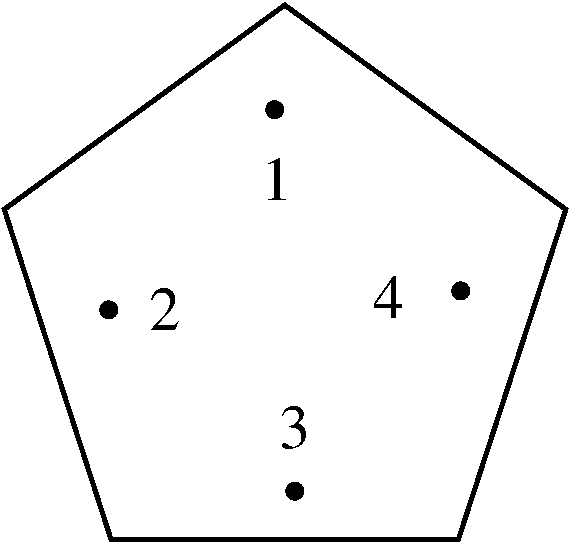
\includegraphics[width=4cm]{figures/pentagon_degree3.pdf}
    \hspace{1cm}
    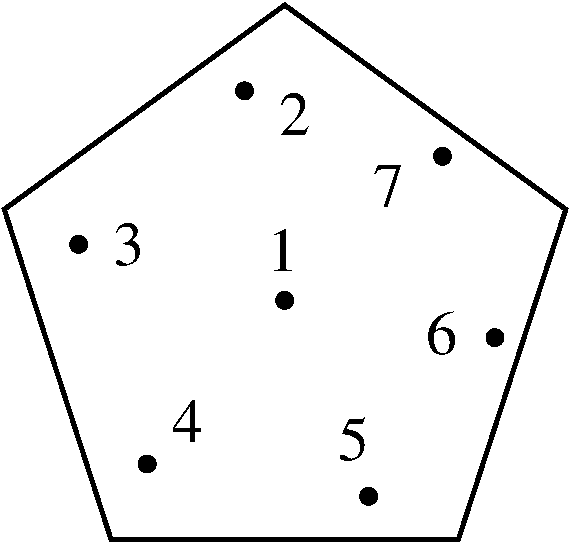
\includegraphics[width=4cm]{figures/pentagon_degree5.pdf}
    \caption{Locations of generalized, Gaussian, quadrature nodes for the $3^{\mathrm{rd}}$ (left) and $5^{\mathrm{th}}$ (right) degree integration methods presented in Table~\ref{tabQuadrature}.  Vertex 1 is located at the top of the pentagon, cf.\ Fig.~\ref{figRegPentagon}, while the coordinate origin is located at its centroid (node 1 in the right figure).  It is readily apparent that these quadrature rules are not symmetric.}
    \label{figQuadrature}
\end{figure}

The Gaussian quadrature rules of Mousavi, Xiao \& Sukumar \cite{Mousavietal10} presented in Table~\ref{tabQuadrature} are compatible with the shape functions of Wachspress \cite{Wachspress75,Wachspress16} and Dasgupta \cite{Dasgupta03} presented in \S\ref{secShapeFns}.  More recently, Chakrabort \textit{et~al}.\ \cite{Chakrabortyetal18} have provided alternative quadrature schemes for pentagons that are also compatible with the Wachspress shape functions.  Again, Table~\ref{tabQuadrature} cannot be found in the literature.

\subsection{Gauss Integration of a Tetrahedron}

Integrating over the volume of a tetrahedron, when expressed in its natural co-ordinates $( \xi , \eta , \zeta )$, which span the ranges of $0 \leq \xi \leq 1$, $0 \leq \eta \leq 1 - \xi$, and $0 \leq \zeta \leq 1 - \xi - \eta$, approximates an integral of some function $f ( \xi , \eta , \zeta )$ as
\begin{multline}
     \mathcal{I} = \int_0^1 \int_{\eta=0}^{1-\xi} \int_{\zeta = 0}^{1 - \xi - \eta} 
     f ( \xi , \eta , \zeta ) \, \mathrm{d} \zeta \, \mathrm{d} \eta \, 
     \mathrm{d} \xi = \sum_{i=1}^n w_i f( \xi_i , \eta_i , \zeta_i ) + E \\
     \text{with} \quad 
     \int_0^1 \int_{\eta=0}^{1-\xi} \int_{\zeta = 0}^{1 - \xi - \eta} 
     \mathrm{d} \zeta \, \mathrm{d} \eta \, \mathrm{d} \xi = \sum_{i=1}^n w_i = 
     \frac{1}{6}
\end{multline}
where co-ordinates $\xi_i$, $\eta_i$ and $\zeta_i$ place the $i^{\text{th}}$ node of integration inside a tetrahedron, and whose corresponding weight of integration is $w_i$, with there being $n$ pairs of nodes and weights.  The volume of this tetradedron is \textfrac{1}{6}.  Table~\ref{tabQuadraturetetra} provides a selection of quadrature rules for tetrahedra when expressed in their natural co-ordinate system.  This table can be found in some finite element textbooks.

\footnotesize
\begin{table}
    \hspace{-1.75cm}
    \begin{tabular}{|c|rrrr|}
        \hline
        node & \centering $\xi$ co-ordinate \phantom{12} & $\eta$ co-ordinate \phantom{12} & 
        $\zeta$ co-ordinate \phantom{12} & weight \phantom{12345} \\ \hline        
        & \multicolumn{4}{|c|}{Exact for Polynomials of Degree $1^{\phantom{|^|}}$} \\ 
        \hline
        1 & 0.250000000000000 & 0.250000000000000 & 0.250000000000000 & 
            0.166666666666667 \\ 
        \hline
        & \multicolumn{4}{|c|}{Exact for Polynomials of Degree $3^{\phantom{|^|}}$} \\ \hline
        1 & 0.250000000000000 & 0.250000000000000 & 0.250000000000000 & 
           -0.133333333333333 \\
        2 & 0.500000000000000 & 0.166666666666667 & 0.166666666666667 &  
            0.075000000000000 \\
        3 & 0.166666666666667 & 0.500000000000000 & 0.166666666666667 &  
            0.075000000000000 \\ 
        4 & 0.166666666666667 & 0.166666666666667 & 0.500000000000000 & 
            0.075000000000000 \\
        5 & 0.166666666666667 & 0.166666666666667 & 0.166666666666667 & 
            0.075000000000000 \\
        \hline
        & \multicolumn{4}{|c|}{Exact for Polynomials of Degree $5^{\phantom{|^|}}$} \\ \hline
        1 & 0.250000000000000 & 0.250000000000000 & 0.250000000000000 &    
            0.030283678097089 \\
        2 & 0.000000000000000 & 0.333333333333333 & 0.333333333333333 & 
            0.006026785714286 \\
        3 & 0.333333333333333 & 0.000000000000000 & 0.333333333333333 & 
            0.006026785714286 \\ 
        4 & 0.333333333333333 & 0.333333333333333 & 0.000000000000000 & 
            0.006026785714286 \\
        5 & 0.333333333333333 & 0.333333333333333 & 0.333333333333333 & 
            0.006026785714286 \\
        6 & 0.727272727272727 & 0.090909090909091 & 0.090909090909091 & 
            0.011645249086029 \\
        7 & 0.090909090909091 & 0.727272727272727 & 0.090909090909091 & 
            0.011645249086029 \\
        8 & 0.090909090909091 & 0.090909090909091 & 0.727272727272727 & 
            0.011645249086029 \\ 
        9 & 0.090909090909091 & 0.090909090909091 & 0.090909090909091 & 
            0.011645249086029 \\
        10 & 0.066550153573664 & 0.433449846426336 & 0.433449846426336 & 
             0.010949141561386 \\
        11 & 0.433449846426336 & 0.066550153573664 & 0.433449846426336 & 
             0.010949141561386 \\
        12 & 0.433449846426336 & 0.433449846426336 & 0.066550153573664 & 
             0.010949141561386 \\
        13 & 0.433449846426336 & 0.066550153573664 & 0.066550153573664 & 
             0.010949141561386 \\ 
        14 & 0.066550153573664 & 0.433449846426336 & 0.066550153573664 & 
             0.010949141561386 \\
        15 & 0.066550153573664 & 0.066550153573664 & 0.433449846426336 & 
             0.010949141561386 \\ 
        \hline
    \end{tabular}
    \caption{Symmetric weights and nodes for Gauss quadratures that integrate over a tetrahedron in its natural co-ordinate system $(\xi , \eta , \zeta)$, where $0 \leq \xi \leq 1 - \eta - \zeta$, $0 \leq \eta \leq 1 - \zeta$ and $0 \leq \zeta \leq 1$.  These weights sum to \textfrac{1}{6}, which is the volume of a tetrahedron measured in its natural co-ordinate system.}
    \label{tabQuadraturetetra}
\end{table}
\normalsize

\section{Interpolation: Nodal Points $\mapsto$ Gauss Points \\ 
         \qquad Extrapolation: Gauss Points $\mapsto$ Nodal Points}
\label{sec:extrapolation}

In a general finite element setting, information comes into the nodes of an element that then gets interpolated down to its Gauss points for their use there.  In many applications, and in particular, in ours, one needs to also be able to take fields, in our case the stress and entropy that have been determined at the Gauss points of an element, and extrapolate this information out to the exterior nodes of the element.

Particular to our application, a suite of nodes is common betwixt three, separate, finite element models comprised of twenty common vertices that belong to a dodecahedron used as a geometric model for an alveolus.  The resultant force at each vertex arises from: a finite element model of thirty 1D rods representing the alveolar chords, a finite element model of twelve 2D pentagons representing the alveolar membranes, and a finite element model of sixty 3D tetrahedra representing the alveolar sac.  The micro\-scopic forces coming from these three models are summed at these twenty common vertices. These resultant forces are then collectively homogenized to yield an averaged macroscopic state of stress for the parenchyma.  Feasibility of this solution strategy hinges upon one's ability to \textit{i\/}) extrapolate stresses evaluated at the Gauss points out to their nodal positions, and \textit{ii\/}) the conversion of these nodal stresses into nodal forces.  We address the first of these two issues in this section, and the second of these two issues in the next section.

Shape functions are introduced for interpolating within an element; specifically, consider an arbitrary field, say $f$, whose values are known at the nodes, then
\begin{subequations}
    \label{extrapolationProcedure}
    \begin{align}
    f ( \boldsymbol{\xi}_k ) & = \sum_{i=1}^n 
    N_i ( \boldsymbol{\xi}_k ) f ( \boldsymbol{x}_i ) &
    k & = 1, 2, \ldots, m 
    \label{interpolation} \\
    \intertext{where the $\boldsymbol{x}_i$ are co-ordinates that locate one of the $n$ vertices in an element of interest, and where the $\boldsymbol{\xi}_i$ are co-ordinates that locate one of its $m$ Gauss points, both being evaluated in the natural co-ordinate system of the element.  Functions $N_i$ are the so-called shape (interpolation) functions.  They obey $\sum_{i=1}^n N_i (\boldsymbol{\xi}) = 1$.
    \bigskip\newline
    A corresponding extrapolation scheme can therefore be written down as}
    f ( \boldsymbol{x}_k ) & = \sum_{i=1}^m 
    M_i ( \boldsymbol{x}_k ) f ( \boldsymbol{\xi}_i ) &
    k & = 1, 2, \ldots, n 
    \label{extrapolation} \\
    \intertext{where the $M_i$ denote extrapolation functions, i.e., they take values of function $f$, now assumed to be known at all Gauss points $\boldsymbol{\xi}_i$, $i=1,2,\ldots,m$, and extrapolate them out to their individual nodal points $\boldsymbol{x}_k$, $k \in \{ 1, 2, \ldots , n \}$. They obey $\sum_{i=1}^m M_i (\boldsymbol{x}) = 1$.
    \bigskip\newline
    These interpolation\slash extrapolation functions must also obey the following constraints: either}
    1 & = \sum_{i=1}^n N_i ( \boldsymbol{\xi}_j )  
    M_j ( \boldsymbol{x}_i ) & j & = 1, 2, \ldots, m 
    \label{extrapolationConstraint1} \\
    0 & = \sum_{i=1}^n N_i ( \boldsymbol{\xi}_j )  
    M_k ( \boldsymbol{x}_i ) & j, k & = 1, 2, \ldots, m , 
    \quad j \neq k
    \label{extrapolationConstraint3}  \\
    \intertext{or}
    1 & = \sum_{i=1}^m  M_i ( \boldsymbol{x}_j )
    N_j ( \boldsymbol{\xi}_i ) & j & = 1, 2, \ldots, n 
    \label{extrapolationConstraint2} \\
    0 & = \sum_{i=1}^m  M_i ( \boldsymbol{x}_j )
    N_k ( \boldsymbol{\xi}_i ) & j, k & = 1, 2, \ldots, n ,
    \quad\; j \neq k
    \label{extrapolationConstraint4}
    \end{align}
\end{subequations}
which follow upon substituting Eqn.~(\ref{extrapolation}) into Eqn.~(\ref{interpolation}), or vice versa.  In this regard, such a pair of interpolation\slash extrapolation functions are self consistent.  

Specifically, whenever $m=n$, the matrices that come about from the interpolation and extrapolation coefficients are reciprocal to one another, with the 0's and 1's of Eqns.~(\ref{extrapolationConstraint1} \& \ref{extrapolationConstraint3} or \ref{extrapolationConstraint2} \& \ref{extrapolationConstraint4}) associating with the individual components of an identity matrix.  Consequently, our need to extrapolate information as-well-as interpolate it strongly suggests that the number of Gauss points selected ought to equal the number of nodal points for any given element geometry.

For example, in the case of a tetrahedron one interpolates via
\begin{subequations}
    \begin{align}
    \left\{ \begin{matrix}
    f ( \boldsymbol{\xi}_1 ) \\ 
    f ( \boldsymbol{\xi}_2 ) \\ 
    f ( \boldsymbol{\xi}_3 ) \\ 
    f ( \boldsymbol{\xi}_4 )
    \end{matrix} \right\} & = \begin{bmatrix}
    N_1 (\boldsymbol{\xi}_1) & N_2 (\boldsymbol{\xi}_1) & 
    N_3 (\boldsymbol{\xi}_1) & N_4 (\boldsymbol{\xi}_1) \\
    N_1 (\boldsymbol{\xi}_2) & N_2 (\boldsymbol{\xi}_2) &
    N_3 (\boldsymbol{\xi}_2) & N_4 (\boldsymbol{\xi}_2) \\
    N_1 (\boldsymbol{\xi}_3) & N_2 (\boldsymbol{\xi}_3) & 
    N_3 (\boldsymbol{\xi}_3) & N_4 (\boldsymbol{\xi}_3) \\
    N_1 (\boldsymbol{\xi}_4) & N_2 (\boldsymbol{\xi}_4) & 
    N_3 (\boldsymbol{\xi}_4) & N_4 (\boldsymbol{\xi}_4)
    \end{bmatrix} \left\{ \begin{matrix} 
    f ( \boldsymbol{x}_1 ) \\ 
    f ( \boldsymbol{x}_2 ) \\ 
    f ( \boldsymbol{x}_3 ) \\
    f ( \boldsymbol{x}_4 ) 
    \end{matrix} \right\}
    \notag \\ 
    \intertext{and extrapolates via}
    \left\{ \begin{matrix} 
    f ( \boldsymbol{x}_1 ) \\ 
    f ( \boldsymbol{x}_2 ) \\ 
    f ( \boldsymbol{x}_3 ) \\
    f ( \boldsymbol{x}_4 )
    \end{matrix} \right\} & = \begin{bmatrix}
    M_1 (\boldsymbol{x}_1) & M_2 (\boldsymbol{x}_1) & 
    M_3 (\boldsymbol{x}_1) & M_4 (\boldsymbol{x}_1) \\
    M_1 (\boldsymbol{x}_2) & M_2 (\boldsymbol{x}_2) &
    M_3 (\boldsymbol{x}_2) & M_4 (\boldsymbol{x}_2) \\
    M_1 (\boldsymbol{x}_3) & M_2 (\boldsymbol{x}_3) & 
    M_3 (\boldsymbol{x}_3) & M_4 (\boldsymbol{x}_3) \\
    M_1 (\boldsymbol{x}_4) & M_2 (\boldsymbol{x}_4) & 
    M_3 (\boldsymbol{x}_4) & M_4 (\boldsymbol{x}_4)
    \end{bmatrix} \left\{ \begin{matrix}
    f ( \boldsymbol{\xi}_1 ) \\ 
    f ( \boldsymbol{\xi}_2 ) \\ 
    f ( \boldsymbol{\xi}_3 ) \\ 
    f ( \boldsymbol{\xi}_4 )
    \end{matrix} \right\}
    \notag
    \end{align}
\end{subequations}
where vectors $\boldsymbol{x}_1$, $\boldsymbol{x}_2$, $\boldsymbol{x}_3$ and $\boldsymbol{x}_4$ hold the co-ordinates of the nodal points, and where vectors $\boldsymbol{\xi}_1$, $\boldsymbol{\xi}_2$, $\boldsymbol{\xi}_3$ and $\boldsymbol{\xi}_4$ hold the co-ordinates of their Gauss points, all evaluated in the natural co-ordinate system of the element.  The matrices in the above mappings are inverses of one another in this construction.
\addtocounter{equation}{-1}

Our three-model finite element analysis of an alveolus requires the use of rods with two nodes, triangles with three nodes, tetrahedra with four nodes, and pentagons with five nodes.  We now provide consistent interpolation\slash extrapolation procedures for these geometries.  This requires the selection of a two-point quadrature rule for rods, a three-point quadrature rule for triangles, a four point quadrature rule for tetrahedra, and a five-point quadrature rule for pentagons.  Our selections, and their associated interpolation\slash extrapolation pairs, are presented below.

\subsection{Self-Consistent Interpolation\slash Extrapolation Procedures for Rods}

Considering a rod with two Gauss points, the interpolation of an arbitrary field, say $f$, whose values are known at nodal points $x_i$, $i=1,2$, into approximated values located at Gauss points $\xi_i$, assigned according to Table~\ref{tab:2nodeRod}, while selecting shape (interpolation) functions $N_1 = \tfrac{1}{2} ( 1 - \xi )$ and $N_2 = \tfrac{1}{2} ( 1 + \xi )$, where $-1 \leq \xi \leq 1$, results in an interpolation that maps values for a field from nodes to Gauss point via
\begin{subequations}
    \begin{align}
     \left\{ \begin{matrix}
    f ( \textfrac{-\sqrt{3}\,}{\,3} ) \\ f ( \textfrac{\sqrt{3}\,}{\,3} )
    \end{matrix} \right\} & = \frac{1}{6} \begin{bmatrix}
        3 + \sqrt{3} & 3 - \sqrt{3} \\
        3 - \sqrt{3} & 3 + \sqrt{3}
    \end{bmatrix} \left\{ \begin{matrix} 
    f ( -1 ) \\ f ( 1 )
    \end{matrix} \right\} 
    \label{interpolateRod} \\
    \intertext{that, upon applying the methodology put forward in Eqn.~(\ref{extrapolationProcedure}), leads to a straight\-forward extrapolation formula that maps values for the field from Gauss points to nodes via}
    \left\{ \begin{matrix} 
    f ( -1 ) \\ f ( 1 )
    \end{matrix} \right\} & 
    = \frac{1}{2 \sqrt{3}} \begin{bmatrix}
    \sqrt{3} + 3 & \sqrt{3} - 3 \\
    \sqrt{3} - 3 & \sqrt{3} + 3
    \end{bmatrix} \left\{ \begin{matrix}
    f ( \textfrac{-\sqrt{3}\,}{\,3} ) \\ f ( \textfrac{\sqrt{3}\,}{\,3} )
    \end{matrix} \right\} .
    \label{extrapolateRod}
    \end{align}
\end{subequations}
This extrapolation matrix can be found in O{\~n}ate \cite[pg.~332]{Onate09}.  As a check, each row in this matrix sums to 1.  Furthermore, the matrices in Eqns.~(\ref{interpolateRod} \& \ref{extrapolateRod}) are reciprocals to one another, as they must be.

\begin{table}
    \begin{center}
        \begin{tabular}{|c|cc|}
            \hline
            node & $\xi$ co-ordinate & weight \\ \hline        
            1 & $-\sqrt{3} / 3^{\vphantom{|^|}}$ & 1 \\ 
            2 & $\phantom{-}\sqrt{3} / 3$ & 1 \\ 
            \hline
        \end{tabular}
    \end{center}
    \caption{A Gauss quadrature rule for integrating functions over the lengths of rods.  It approximates $\int_{-1}^1 f(\xi) \, \mathrm{d}\xi$ using two quadrature points.  The weights of quadrature sum to its length because $L = \int_{-1}^1 \mathrm{d} \xi = 2$.  This quadrature rule is from Christoffel.  It integrates polynomials along a line exactly up through second order.}
    \label{tab:2nodeRod}
\end{table}

\subsection{Self-Consistent Interpolation\slash Extrapolation Procedures for Triangles}

Now, considering a triangle with three Gauss points, the interpolation of an arbitrary field $f$ whose values are known at nodal points $\boldsymbol{x}_i$, $i=1,2,3$, into approximated values located at Gauss points $\boldsymbol{\xi}$, assigned according to Table~\ref{tab:3nodeTriangle}, while selecting shape (interpolation) functions $N_1 = 1 - \xi - \eta$, $N_2 = \xi$, and $N_3 = \eta$, where $0 \leq \xi \leq 1$ and $0 \leq \eta \leq 1 - \xi$, results in an interpolation that maps according to
\begin{subequations}
    \begin{align}
    \left\{ \begin{matrix}
    f ( \textfrac{1}{6} , \textfrac{1}{6} ) \\ 
    f ( \textfrac{2}{3} , \textfrac{1}{6} ) \\ 
    f ( \textfrac{1}{6} , \textfrac{2}{3} )
    \end{matrix} \right\} & = \frac{1}{6} \begin{bmatrix}
    4 & 1 & 1 \\
    1 & 4 & 1 \\
    1 & 1 & 4
    \end{bmatrix} \left\{ \begin{matrix} 
    f ( 0, 0 ) \\ f ( 1, 0 ) \\ f ( 0, 1 )
    \end{matrix} \right\}
    \label{interpolateTriangle} \\
    \intertext{that, upon applying the methodology put forward in Eqn.~(\ref{extrapolationProcedure}), which requires some algebra, leads to a simple extrapolation formula applicable for triangles when evaluated in their natural co-ordinate system, viz.,}
    \left\{ \begin{matrix} 
    f ( 0, 0 ) \\ f ( 1, 0 ) \\ f ( 0, 1 )
    \end{matrix} \right\} & 
    = \frac{1}{3} \begin{bmatrix}
        5 & -1 & -1 \\
        -1 & 5 & -1 \\
        -1 & -1 & 5
    \end{bmatrix} \left\{ \begin{matrix}
        f ( \textfrac{1}{6} , \textfrac{1}{6} ) \\ 
        f ( \textfrac{2}{3} , \textfrac{1}{6} ) \\ 
        f ( \textfrac{1}{6} , \textfrac{2}{3} )
    \end{matrix} \right\} .
    \label{extrapolateTriangle}
    \end{align}
\end{subequations}
As a check, each row in both matrices sums to 1 and, as expected, plus these matrices are reciprocals to one another.

\begin{table}
    \begin{center}
    \begin{tabular}{|c|ccc|}
        \hline
        node & $\xi$ co-ordinate & $\eta$ co-ordinate  & weight \\ \hline        
        1 & 1/6 & 1/6 & 1/6 \\ 
        2 & 2/3 & 1/6 & 1/6 \\ 
        3 & 1/6 & 2/3 & 1/6 \\ 
        \hline
    \end{tabular}
    \end{center}
    \caption{A Gauss quadrature rule for integrating functions over the areas of triangles.  It approximates $\int_0^1 \int_0^{1-\xi} f(\xi , \eta) \, \mathrm{d} \eta \, \mathrm{d} \xi$  using three quadrature points.  The weights of quadrature sum to its area because $A = \int_0^1 \int_0^{1-\xi} \mathrm{d}\eta \, \mathrm{d} \xi = \textfrac{1}{2}$.  This quadrature rule is from Strang.  It integrates polynomials over a triangular region exactly up through second order.}
    \label{tab:3nodeTriangle}
\end{table}
    
\subsection{Self-Consistent Interpolation\slash Extrapolation Procedures for Tetrahedra}
    
We now consider a tetrahedron with four Gauss points.  Here the interpolation of an arbitrary field $f$ whose values are known at nodal points $\boldsymbol{x}_i$, $i=1,2,3,4$, into approximated values located at Gauss points $\boldsymbol{\xi}_i$, assigned according to Table~\ref{tab:4nodedTet}, while selecting shape functions $N_1 = 1 - \xi - \eta - \zeta$, $N_2 = \xi$, $N_3 = \eta$, and $N_4 = \zeta$, bounded by $0 \leq \xi \leq 1$, $0 \leq \eta \leq 1 - \xi$ and $0 \leq \zeta \leq 1 - \xi - \eta$, leads to the following interpolation formula
\begin{subequations}
    \label{extrapolationTetrahedron}
    \begin{align}
         \left\{ \begin{matrix}
        f ( a, a, a ) \\ 
        f ( b, a, a ) \\ 
        f ( a, b, a ) \\
        f ( a, a, b )
        \end{matrix} \right\} & = \begin{bmatrix}
        1 - 3a & a & a & a \\
        1-2a-b & b & a & a \\
        1-2a-b & a & b & a \\
        1-2a-b & a & a & b
        \end{bmatrix} \left\{ \begin{matrix} 
        f ( 0, 0, 0) \\ f ( 1, 0, 0 ) \\ f ( 0, 1, 0 ) \\ f ( 0, 0, 1 )
        \end{matrix} \right\} 
        \label{interpolateTet} \\
    \intertext{that, upon applying the methodology put forward in Eqn.~(\ref{extrapolationProcedure}), which now requires a good deal of algebra, results in the following extrapolation formula for tetrahedra}
    \left\{ \begin{matrix} 
        f ( 0, 0, 0) \\ f ( 1, 0, 0 ) \\ f ( 0, 1, 0 ) \\ f ( 0, 0, 1 )
        \end{matrix} \right\} & 
    = \frac{1}{b-a}\begin{bmatrix}
        2a+b & -a & -a & -a \\
        2a+b-1 & 1-a & -a & -a \\
        2a+b-1 & -a & 1-a & -a \\
        2a+b-1 & -a & -a & 1-a
    \end{bmatrix} \left\{ \begin{matrix}
        f ( a, a, a ) \\ 
        f ( b, a, a ) \\ 
        f ( a, b, a ) \\
        f ( a, a, b )
    \end{matrix} \right\} 
    \label{extrapolateTet}
    \end{align}
\end{subequations}
where $a = 0.1381966011250105$ and $b = 0.5854101966249685$ from Table~\ref{tab:4nodedTet}.  As a check, each row in the above matrices sums to 1.  Unlike the interpolation\slash extrapolation formul\ae\ for rods and triangles, whose matrices are symmetric, here these matrices of interpolation\slash extrapolation coefficients are not symmetric. 
    
\begin{table}
    \hspace{-7mm}
    \begin{tabular}{|c|cccc|}
        \hline
        node & $\xi$ co-ordinate & $\eta$ co-ordinate & 
        $\zeta$ co-ordinate & weight \\ \hline        
        1 & 0.1381966011250105 & 0.1381966011250105 & 0.1381966011250105 & 1/24 \\
        2 & 0.5854101966249685 & 0.1381966011250105 & 0.1381966011250105 & 1/24 \\
        3 & 0.1381966011250105 & 0.5854101966249685 & 0.1381966011250105 & 1/24 \\
        4 & 0.1381966011250105 & 0.1381966011250105 & 0.5854101966249685 & 1/24 \\
        \hline
    \end{tabular}
    \caption{A Gauss quadrature rule for integrating functions over the volumes of tetrahedra.  It approximates $\int_0^1 \int_0^{1-\xi} \int_0^{1-\xi-\eta} f(\xi, \eta, \zeta) \, \mathrm{d}\zeta \, \mathrm{d}\eta \, \mathrm{d}\xi$ using four quadrature points.  The weights of quadrature sum to its volume because $V = \int_0^1 \int_0^{1-\xi} \int_0^{1-\xi-\eta} \mathrm{d}\zeta \, \mathrm{d}\eta \, \mathrm{d}\xi = \textfrac{1}{6}$.  This quadrature rule is from Keast.  It integrates polynomials over a tetrahedral region exactly up through second order.  As a point of reference, the centroid has co-ordinates (\textfrac{1}{4}, \textfrac{1}{4}, \textfrac{1}{4}).}
    \label{tab:4nodedTet}
\end{table}

\subsection{Self-Consistent Interpolation\slash Extrapolation Procedures for Pentagons}

We only know of two papers where quadrature formul\ae\ have been created for integrating over the area of pentagons. \cite{Mousavietal10,Chakrabortyetal18}  Neither presents tables for their nodes and weights of quadrature, cf.\ \S\ref{sec:pentagonQuadrature} for such a table.  Only mathematical methodologies from which one can numerically construct such tables are published.  Also, neither of their strategies exploits the symmetry properties of a pentagon.  

Because we seek a quadrature rule for regular pentagons that employs five Gauss points, and pentagons posses five radial lines of symmetry, it is reasonable to consider that the five nodes of quadrature that we seek lie along these five radial lines.  Specifically, we seek a quadrature rule for a pentagon whose vertices are located at $\boldsymbol{x}_i$, $i=1,2,\ldots,5$, and whose nodes of quadrature are located at $\boldsymbol{\xi}_i$ such that
\begin{subequations}
    \label{pentagonCoordinates}
    \begin{align}
    \boldsymbol{x}_1 & = \bigl( \cos ( \textfrac{\pi}{2} ) ,
        \sin ( \textfrac{\pi}{2} ) \bigr) & \boldsymbol{\xi}_1 & = \ell \boldsymbol{x}_1 \\
    \boldsymbol{x}_2 & = \bigl( \cos ( \textfrac{9\pi}{10}) ,
    \sin ( \textfrac{9\pi}{10} ) \bigr) & \boldsymbol{\xi}_2 & = \ell \boldsymbol{x}_2 \\
    \boldsymbol{x}_3 & = \bigl( \cos ( \textfrac{13\pi}{10}) ,
    \sin ( \textfrac{13\pi}{10} ) \bigr) & \boldsymbol{\xi}_3 & = \ell \boldsymbol{x}_3 \\
    \boldsymbol{x}_4 & = \bigl( \cos ( \textfrac{17\pi}{10}) ,
    \sin ( \textfrac{17\pi}{10} ) \bigr) & \boldsymbol{\xi}_4 & = \ell \boldsymbol{x}_4 \\
    \boldsymbol{x}_5 & = \bigl( \cos ( \textfrac{\pi}{10}) ,
    \sin ( \textfrac{\pi}{10} ) \bigr) & \boldsymbol{\xi}_5 & = \ell \boldsymbol{x}_5
    \end{align}
\end{subequations}
where lines radiating from the origin out to vertices $\boldsymbol{x}_i$ each have unit length, while those that radiate out to the Gauss points $\boldsymbol{\xi}$ have a shorter length of $\ell$.

Implementing the strategies that underlie Gauss quadrature, length $\ell$ represents a distance out to the centroid of an area.  In our case, this area (one of five equivalent areas) is a four-sided polygon whose apex has an inside angle of $108^{\circ}$, whose shoulders have right angles, and whose inside angle at the origin is $72^{\circ}$.  A little bit of geometry and algebra leads to the result that
\begin{subequations}
    \label{pentagonQuadrature}
    \begin{align}
    \ell & = \frac{1 + \sin ( \textfrac{3\pi}{10} )}
    {3 \sin ( \textfrac{3\pi}{10} ) } \approx 0.7454 \\
    \intertext{whose associated area becomes the weight of quadrature}
    w & = \sin ( \textfrac{3\pi}{10} ) \cos ( \textfrac{3\pi}{10} ) 
    \approx 0.4755 
    \end{align}
\end{subequations}
which is one-fifth the area of a pentagon, cf.\ Eqn.~(\ref{regPentagonArea}).  To the best of our knowledge, the quadrature rule put forward in Eqns.~(\ref{pentagonCoordinates} \& \ref{pentagonQuadrature}) for regular pentagons is new to the literature. 

Interpolation is described through shape functions.  Adopting the shape functions of Wachspress, which were constructed in \S\ref{secShapeFns} for a pentagon, while using the quadrature rule of Eqns.~(\ref{pentagonCoordinates} \& \ref{pentagonQuadrature}), results in a symmetric interpolation map of
\begin{subequations}
    \label{extrapolationPentagon}
    \begin{align} 
    \left\{ \begin{matrix}
    f ( \boldsymbol{\xi}_1 ) \\ 
    f ( \boldsymbol{\xi}_2 ) \\ 
    f ( \boldsymbol{\xi}_3 ) \\ 
    f ( \boldsymbol{\xi}_4 ) \\ 
    f ( \boldsymbol{\xi}_5 )
    \end{matrix} \right\} & = \begin{bmatrix}
    a & b & c & c & b \\
    b & a & b & c & c \\
    c & b & a & b & c \\
    c & c & b & a & b \\
    b & c & c & b & a
    \end{bmatrix} 
    \left\{ \begin{matrix} 
    f ( \boldsymbol{x}_1 ) \\ 
    f ( \boldsymbol{x}_2 ) \\ 
    f ( \boldsymbol{x}_3 ) \\
    f ( \boldsymbol{x}_4 ) \\
    f ( \boldsymbol{x}_5 )
    \end{matrix} \right\} \\
    \intertext{with elements sized as $a = 0.6901471673508344$, $b = 0.1367959452017669$ and $c = 0.0181304711228159$, and an ensueing extrapolation map that is described by}
    \left\{ \begin{matrix} 
    f ( \boldsymbol{x}_1 ) \\ 
    f ( \boldsymbol{x}_2 ) \\ 
    f ( \boldsymbol{x}_3 ) \\
    f ( \boldsymbol{x}_4 ) \\
    f ( \boldsymbol{x}_5 )
    \end{matrix} \right\} & = \frac{1}{\Delta} \begin{bmatrix}
    x & y & z & z & y \\
    y & x & y & z & z \\
    z & y & x & y & z \\
    z & z & y & x & y \\
    y & z & z & y & x
    \end{bmatrix} \left\{ \begin{matrix}
    f ( \boldsymbol{\xi}_1 ) \\ 
    f ( \boldsymbol{\xi}_2 ) \\ 
    f ( \boldsymbol{\xi}_3 ) \\ 
    f ( \boldsymbol{\xi}_4 ) \\ 
    f ( \boldsymbol{\xi}_5 )
    \end{matrix} \right\}  \\
    \intertext{wherein}
    x & = a^2 + (a-b)(b+c) - c^2 \\
    y & = (b+c)c - (a+b)b \\
    z & = b^2 - (a-b)c - c^2 \\
    \Delta & = a^2 - (a+b)b - (a-3b)c - c^2
    \end{align}
\end{subequations}
where, as a check, $\sum_{i=1}^5 N_i (\boldsymbol{\xi}_j) = 1$ and $\sum_{i=1}^5 M_i (\boldsymbol{x}_j) = 1$ for $j=1,2,\ldots,5$, and therefore, $a + 2b + 2c = 1$ and $x + 2y + 2z = \Delta$.  Furthermore, these coefficient matrices for interpolation and extrapolation are inverses to one another.  


\section{Converting Nodal Stresses into Nodal Forces}


